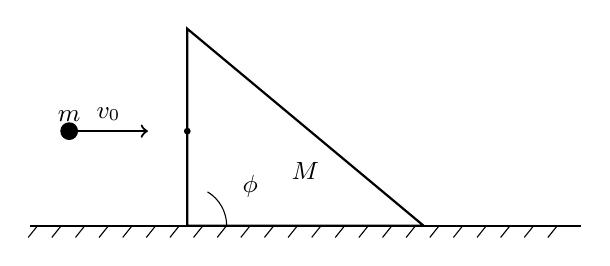
\begin{tikzpicture}[font=\small]
  % 小球水平速度v₀碰撞斜面体
  % 光滑水平面
  \draw[thick] (-1,0) -- (6,0);
  \foreach \x in {-0.9,-0.6,...,5.9}
    \draw (\x,0) -- (\x-0.12,-0.15);
  % 斜面体
  \draw[thick] (1,0) -- (4,0) -- (1,2.5) -- cycle;
  \node at (2.5,0.7) {$M$};
  % 斜面倾角φ
  \draw (1.5,0) arc[start angle=0, end angle=59, radius=0.5];
  \node at (1.8,0.5) {$\phi$};
  % 小球
  \filldraw (-0.5,1.2) circle (3pt) node[above] {$m$};
  % 小球速度
  \draw[->, thick] (-0.5,1.2) -- (0.5,1.2) node[midway, above] {$v_0$};
  % 碰撞点
  \filldraw (1,1.2) circle (1pt);
\end{tikzpicture}
